
\documentclass{beamer}
\usepackage{tikz}
\usetheme{Berkeley}
\usecolortheme{default}

\title{Car Configuration Ontology}
\author{Andrei Rusu, Bogdan Dragoteanu}
\institute{Technical University of Cluj-Napoca}
\date{May 2021}

\begin{document}

\frame{\titlepage}

\begin{frame}
\frametitle{Table of Contents}
\tableofcontents
\end{frame}

% ----- CQs and Use Cases -----
\section{CQs and Use Cases}

% ----------
\begin{frame}{Table of Contents}
    \tableofcontents[currentsection]
\end{frame}

% ----------
\begin{frame}

\frametitle{Competency Questions}

We have compiled the following list of Competency Questions:

\begin{itemize}
\item Is item X compatible with model Y?
\item Is item X compatible only with model Y?
\item What models are compatible with item X?
\item Is item X1 compatible with item X2?
\item Is item X standard or optional?
\item Is model Y an electric vehicle?
\item What interior trim options are there for model Y?
\item Does item X1 include item X2?
\item Is item X an interior or exterior item?
\item Is model Y available with large wheels?
\item Is a glass roof available for model Y?
\end{itemize}
\end{frame}

% ----------
\begin{frame}
\frametitle{Use Cases}
\begin{itemize}
    \item Finding out which configuration items are compatible with the desired vehicle
    \item Checking the compatibility configuration items between themselves
\end{itemize}
\end{frame}

% ----------
% \begin{frame}
% \frametitle{Sample frame title}

% In this slide, some important text will be
% \alert{highlighted} because it's important.
% Please, don't abuse it.

% \begin{block}{Remark}
% Sample text
% \end{block}

% \begin{alertblock}{Important theorem}
% Sample text in red box
% \end{alertblock}

% \begin{examples}
% Sample text in green box. The title of the block is ``Examples".
% \end{examples}
% \end{frame}


% ----- TBox -----
\section{TBox}
\begin{frame}{Table of Contents}
    \tableofcontents[currentsection]
\end{frame}

\begin{frame}{Engine Options}
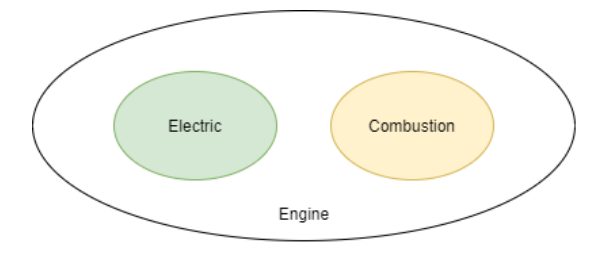
\includegraphics[\centering]{engine.png}
\end{frame}

\begin{frame}{Exterior Options}
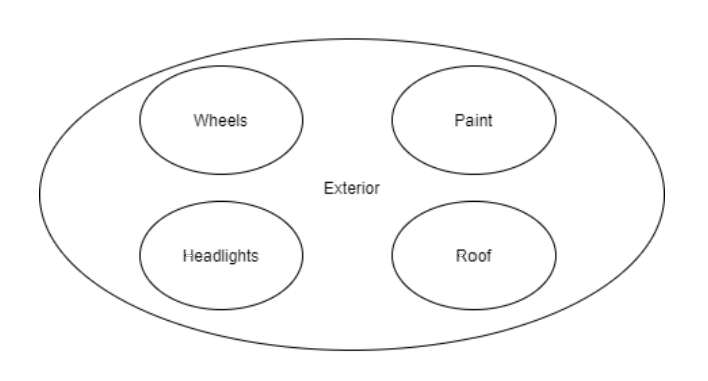
\includegraphics[\centering]{exterior.png}
\end{frame}

\begin{frame}{Interior Options}
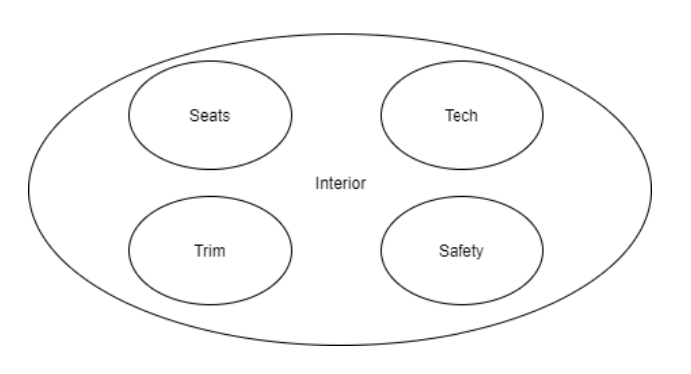
\includegraphics[\centering]{interior.png}
\end{frame}

\begin{frame}{Taxonomy}
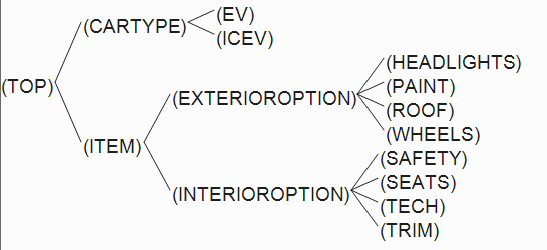
\includegraphics[\centering]{Taxonomy.png}
\end{frame}


% ----- ABox -----
\section{ABox}
\begin{frame}{Table of Contents}
    \tableofcontents[currentsection]
\end{frame}

\begin{frame}{Exterior Items}
\begin{block}{Instances}
; --- WHEELS ---
    
(instance Wheels19 Wheels)

(instance Wheels20 Wheels)

(instance Wheels21 Wheels)

; --- PAINT ---

(instance MetallicPaint Paint)

(instance PearlescentPaint Paint)

; --- HEADLIGHTS ---

(instance LEDLights Headlights)

(instance MatrixLEDLights Headlights)

; --- ROOF ---

(instance CarbonRoof Roof)

(instance GlassRoof Roof)

(instance PanoramicRoof Roof)
\end{block}

\end{frame}

\begin{frame}{Interior Items}
\begin{block}{Instances}
; --- SEATS ---

(instance HeatedSeats Seats)

(instance HeatedSeats (equal isOptional 1))

(instance HeatedSeats (equal hasPrice 500))

(instance RegularSeats Seats)

(instance RegularSeats (equal isOptional 0))

(instance RegularSeats (equal hasPrice 0))

(instance SportSeats Seats)

; --- TECH ---

(instance ElectricBoot Tech)

(instance Camera Tech)

(instance ACC Tech)

(instance FullTechPack Tech)

(instance StarterTechPack Tech)
\end{block}
\end{frame}

\begin{frame}{Interior Items}
\begin{block}{Instances}
; --- TRIM ---

(instance MetalTrim Trim)

(instance WoodTrim Trim)

(instance RegularLeather Trim)

(instance NappaLeather Trim)

; --- SAFETY ---

(instance BlindSpotMonitor Safety)

(instance BlindSpotMonitor (equal isOptional 1))

(instance BlindSpotMonitor (equal hasPrice 300))

(instance FullSafetySystem Safety)

(instance FullSafetySystem (equal isOptional 1))

(instance FullSafetySystem (equal hasPrice 900))

(instance ParkingSensors Safety)

(instance ParkingAssistant Safety)
\end{block}
\end{frame}

\begin{frame}{Taycan Vehicle}
    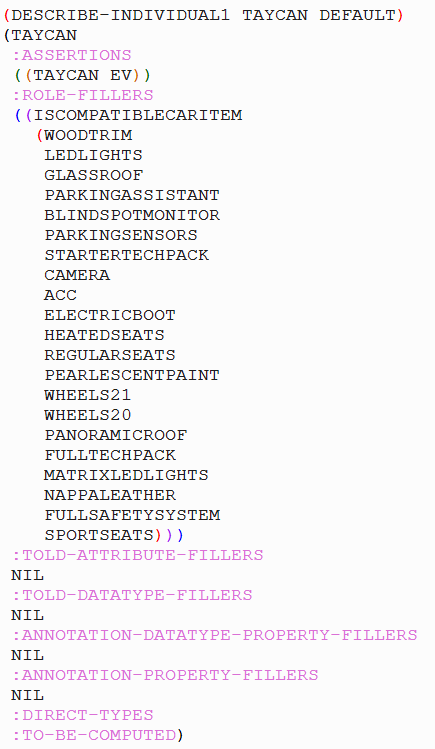
\includegraphics[height=\textheight,keepaspectratio]{taycan.png}
\end{frame}

\begin{frame}{Macan Vehicle}
    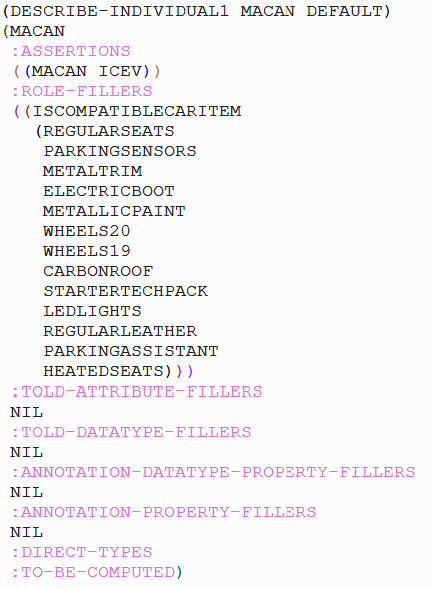
\includegraphics[height=\textheight,keepaspectratio]{macan.png}
\end{frame}

\begin{frame}{Packs \& Inclusions}
; Seats packs
    
(related RegularSeats HeatedSeats isIncluded)

(related HeatedSeats SportSeats isIncluded)

; Light packs

(related LEDLights MatrixLEDLights isIncluded)

; Roof packs

(related GlassRoof PanoramicRoof isIncluded)

; Tech packs

(related ElectricBoot StarterTechPack isIncluded)

(related StarterTechPack FullTechPack isIncluded)

(related Camera FullTechPack isIncluded)

(related ACC FullTechPack isIncluded)
\end{frame}

\begin{frame}{Packs \& Inclusions}
; Trim packs

(related MetalTrim RegularLeather isIncluded)

(related WoodTrim NappaLeather isIncluded)

; Safety Packs

(related ParkingSensors ParkingAssistant isIncluded)

(related ParkingAssistant FullSafetySystem isIncluded)

(related BlindSpotMonitor FullSafetySystem isIncluded)
\end{frame}

\begin{frame}{Visual Representation}
    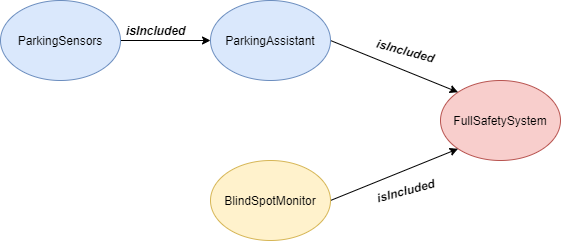
\includegraphics[width=\textwidth]{EquipmentPack.png}
\end{frame}

% ----- Roles -----
\section{Roles}
\begin{frame}{Table of Contents}
    \tableofcontents[currentsection]
\end{frame}

\begin{frame}{Roles}
\begin{itemize}
    \item isCompatibleCarItem
    \item isCompatibleItemItem
    \item isIncluded
\end{itemize}
\end{frame}

\begin{frame}{Role Definitions}
\textit{isCompatibleCarItem :domain CarType :range Item}

\textit{isCompatibleItemItem :domain Item :range Item :symmetric t}

\textit{isIncluded :domain Item :range Item :asymmetric t}
\end{frame}

\begin{frame}{Domain Attributes}
\textit{(define-concrete-domain-attribute hasPrice :type integer)}

\textit{(define-concrete-domain-attribute isOptional :type integer)}
\end{frame}

% ----- Rules -----
\section{Rules}
\begin{frame}{Table of Contents}
    \tableofcontents[currentsection]
\end{frame}

\begin{frame}{Inclusion Compatibility}
    \textit{(define-rule (?car ?item2 isCompatibleCarItem)}
    
    \textit{(and (?car CarType) (?item1 Item) (?item2 Item) (not (same-as ?item1 ?item2))}
    
    \textit{(?car ?item1 isCompatibleCarItem) (?item2 ?item1 isIncluded))) }
    
    \begin{block}{Explanation}
        If a car is compatible with an item that includes another item, the car is also compatible with that other item.
    \end{block}
     
\end{frame}

\begin{frame}{Item Compatibility}
    \textit{(define-rule (?item1 ?item3 isIncluded)}
    
    \textit{(and (?item1 Item) (?item2 Item) (?item3 Item) (not (same-as ?item1 ?item2)) (not (same-as ?item2 ?item3)) (not (same-as ?item1 ?item3))}
    
    \textit{(?item1 ?item2 isIncluded) (?item2 ?item3 isIncluded))) }
    
    \begin{block}{Explanation}
        If item1 is included in item2 and item2 is included in item3, item1 is included in item3 (transitivity).
    \end{block}
     
\end{frame}

% ----- Ontology Design Patterns -----
\section{Ontology Design Patterns}
\begin{frame}{Table of Contents}
    \tableofcontents[currentsection]
\end{frame}

\begin{frame}{Set}
    Used to model sets of elements that are all unique.
    \begin{examples}
        All item categories (both interior and exterior)
    \end{examples}
\end{frame}

\begin{frame}{ViewInheritance}
    Used to model abstraction.
    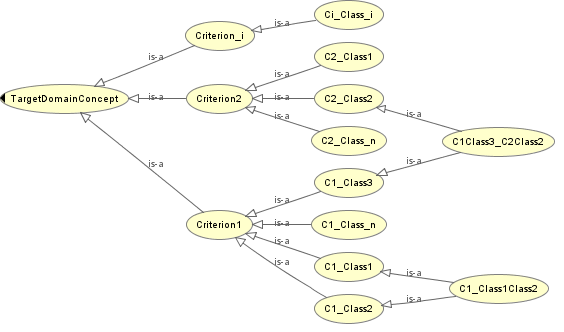
\includegraphics[width=0.7\textwidth ,keepaspectratio]{Fig_view_inheritance_structure.png}
    \begin{examples}
        Only instances of sub-categories, not abstract categories (Wheels not ExteriorItem)
    \end{examples}
    
\end{frame}

\begin{frame}{Parameter}
    Used to model characteristics of concepts.
    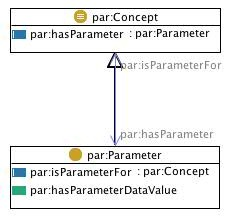
\includegraphics[width=0.4\textwidth ,keepaspectratio]{Parameter.jpg}
    \begin{examples}
        Price and optionality of components (hasPrice \& isOptional).
    \end{examples}
\end{frame}

\begin{frame}{PartOf}
    Used to model entities and their component parts.
    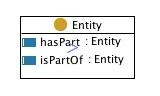
\includegraphics[width=0.4\textwidth ,keepaspectratio]{Partof.jpg}
    \begin{examples}
        Equipment packs that are made up of other components.
    \end{examples}
\end{frame}

% ----- Racer Java API -----
\section{Racer Java API}
\begin{frame}{Table of Contents}
    \tableofcontents[currentsection]
\end{frame}

\begin{frame}{JRacer}
    The library used to communicate with Racer from Java.
    \includegraphics[width=0.4\textwidth ,keepaspectratio]{folders.png}
\end{frame}

\begin{frame}{Establishing a connection}
    The method of connecting the Racer backend to the Java application
    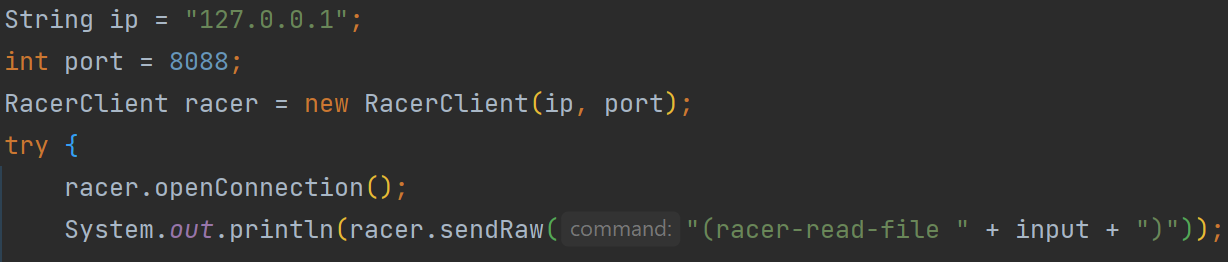
\includegraphics[width=1.0\textwidth ,keepaspectratio]{connection.png}
\end{frame}

\begin{frame}{Java Code}
    Performs the actual work
    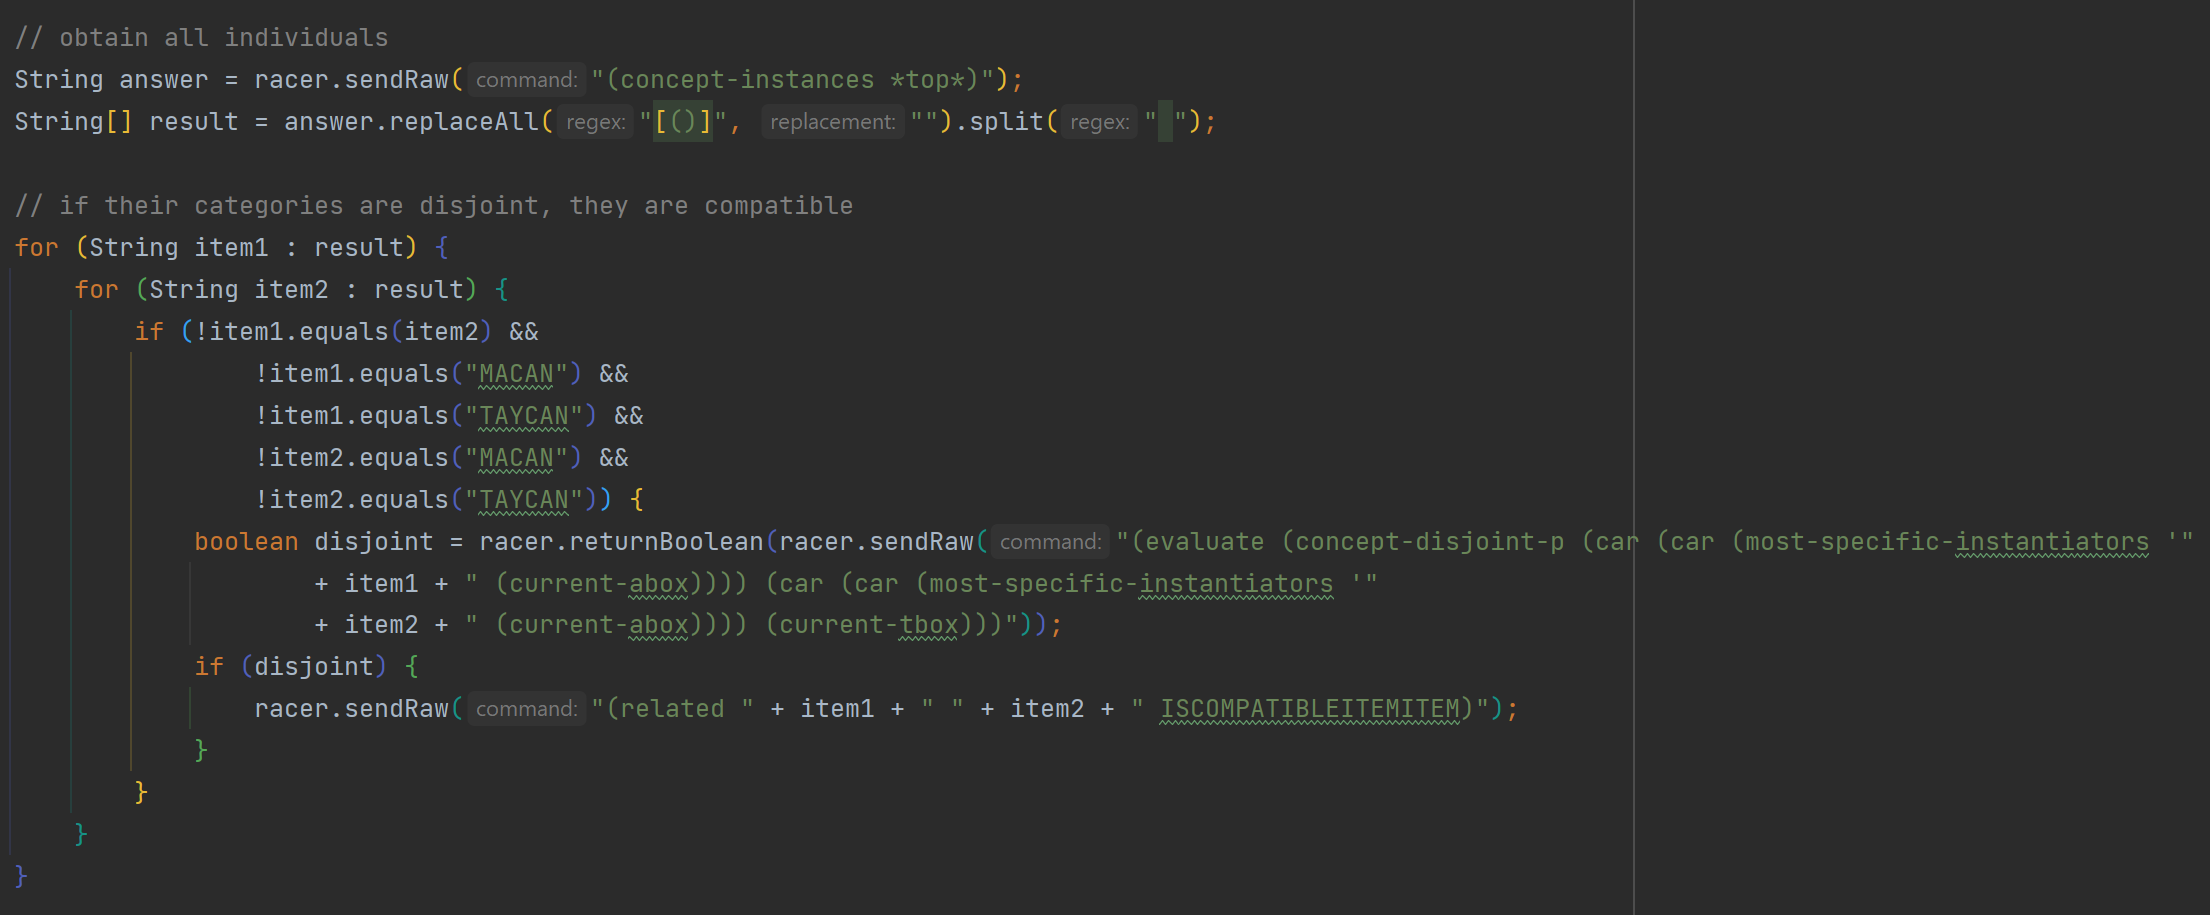
\includegraphics[width=1.0\textwidth ,keepaspectratio]{javacode1.png}
    \begin{block}{Explanation}
        Infers item-to-item compatibility based on their categories.
    \end{block}
\end{frame}

% ----- FuzzyDL -----
\section{FuzzyDL}
\begin{frame}{Table of Contents}
    \tableofcontents[currentsection]
\end{frame}

\begin{frame}{Steps}
    \begin{itemize}
        \item We wanted to express how expensive a component is
        \item We created the file ”FuzzyCar.txt” which contains the concepts, intances and interogations in Fuzzy DL.
        \item We downloaded from http://www.umbertostraccia.it/cs/software/fuzzyDL/fuzzyDL.html
        \item We accessed the folder in which the .jar and ”FuzzyCar.txt” reside
        \item We opened the cmd terminal by typing cmd into the file path area (Windows) and ran the following command: \textit{java -jar FuzzyDL.jar FuzzyCar.txt}
    \end{itemize}
\end{frame}

\begin{frame}{Results}
    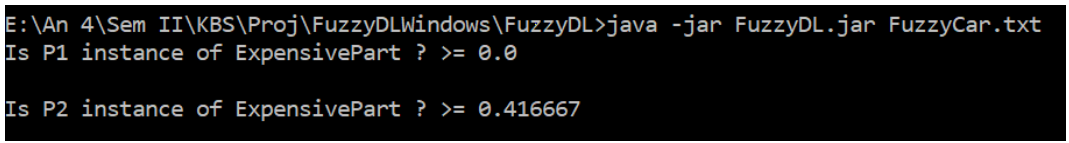
\includegraphics[width=1.0\textwidth ,keepaspectratio]{fuzzy.png}
\end{frame}

\begin{frame}{Code}
(define-modifier very linear-modifier(0.8))

(define-fuzzy-concept Part1PriceRange crisp(0,10000,80,1500))

(define-fuzzy-concept Part2PriceRange crisp(0,10000,6000,10000))

(define-fuzzy-concept Expensive right-shoulder(0,10000,4000,10000))

(define-concept ExpensivePart (and Part (some Price (very Expensive)))) 

(instance P1 (and Part (some Price Part1PriceRange)) 1)

(instance P2 (and Part (some Price Part2PriceRange)) 1)

(min-instance? P1 ExpensivePart)

(min-instance? P2 ExpensivePart)
\end{frame}

% ----- Queries -----
\section{Queries}

\begin{frame}{Racer Queries}
\begin{examples}
    (related-individuals isCompatibleCarItem)

(related-individuals isCompatibleItemItem)

(related-individuals isIncluded)

(individual-fillers Taycan isCompatibleCarItem)

(concept-disjoint? Wheels Tech)

(individuals-related? ParkingSensors FullSafetySystem isIncluded)

(evaluate (> (retrieve-individual-told-attribute-value 'HeatedSeats 'hasPrice (current-abox))
\end{examples}

\end{frame}

\begin{frame}{Racer Queries}
    \begin{examples}
        
(retrieve-individual-told-attribute-value 'RegularSeats 'hasPrice (current-abox))))

(individuals-related? Taycan BlindSpotMonitor isCompatibleCarItem)

(individuals-related? Taycan ParkingSensors isCompatibleCarItem)

(individuals-related? BlindSpotMonitor Wheels19 isCompatibleItemItem)

(retrieve-individual-told-attribute-value 'HeatedSeats 'isOptional (current-abox))
    \end{examples}
\end{frame}

\begin{frame}{NRQL Queries}
\begin{examples}
(get-nrql-version)
    
(enable-nrql-warnings)

(defquery is-interior (?x) (or (?x Seats) (?x Safety) (?x Tech) (?x Trim)))

(defquery is-included (?x ?y) (?x ?y isIncluded))

; all interior items
(retrieve (?x) (?x is-interior))

; items included in other items
(retrieve (?x ?y) (?x ?y is-included))

\end{examples}
\end{frame}

\begin{frame}{NRQL Queries}
\begin{examples}
; interior trim for Taycan

(defquery trim-options (?car ?trim) (and (?car CarType) (?trim Trim) (?car ?trim isCompatibleCarItem)))

(retrieve (?trim) (Taycan ?trim trim-options))

; models compatible with an item

(defquery compat-cars (?car ?item) (and (?car CarType) (?item Item) (?car ?item isCompatibleCarItem)))

(retrieve (?car) (?car SportSeats compat-cars))
\end{examples}
\end{frame}

\begin{frame}{Racer Query Results}
    Racer Message (STDOUT):(ABOX-CONSISTENT?) \rightarrow T
    
(TBOX-CYCLIC?) \rightarrow NIL

(TBOX-COHERENT?) \rightarrow T

(EVALUATE (LENGTH (ALL-INDIVIDUALS))) \rightarrow 28

(EVALUATE (LENGTH (ALL-ATOMIC-CONCEPTS))) \rightarrow 16

(EVALUATE (LENGTH (ALL-ROLES))) \rightarrow 12

(EVALUATE (LENGTH (ALL-RULES))) \rightarrow 2
\end{frame}

\begin{frame}{Racer Query Results}
(GET-TBOX-LANGUAGE) \rightarrow 'L-C-RI'
    
(GET-ABOX-LANGUAGE) \rightarrow 'L-C-RI(D)'

(RELATED-INDIVIDUALS ISCOMPATIBLECARITEM) \rightarrow ((MACAN REGULARSEATS) (MACAN PARKINGSENSORS) ... )

(RELATED-INDIVIDUALS ISCOMPATIBLEITEMITEM) \rightarrow ((WOODTRIM MATRIXLEDLIGHTS) (WOODTRIM PANORAMICROOF) ... )

(RELATED-INDIVIDUALS ISINCLUDED) \rightarrow ((WOODTRIM NAPPALEATHER) (LEDLIGHTS MATRIXLEDLIGHTS) ... )

(INDIVIDUAL-FILLERS TAYCAN ISCOMPATIBLECARITEM) \rightarrow (SPORTSEATS FULLSAFETYSYSTEM NAPPALEATHER MATRIXLEDLIGHTS ... )

(CONCEPT-DISJOINT? WHEELS TECH) \rightarrow T

\end{frame}

\begin{frame}{Racer Query Results}
    (INDIVIDUALS-RELATED? PARKINGSENSORS FULLSAFETYSYSTEM ISINCLUDED) \rightarrow T

(EVALUATE (> (RETRIEVE-INDIVIDUAL-TOLD-ATTRIBUTE-VALUE (QUOTE HEATEDSEATS) (QUOTE HASPRICE) (CURRENT-ABOX)) (RETRIEVE-INDIVIDUAL-TOLD-ATTRIBUTE-VALUE (QUOTE REGULARSEATS) (QUOTE HASPRICE) (CURRENT-ABOX)))) \rightarrow T

(INDIVIDUALS-RELATED? TAYCAN BLINDSPOTMONITOR ISCOMPATIBLECARITEM) \rightarrow T

(INDIVIDUALS-RELATED? TAYCAN PARKINGSENSORS ISCOMPATIBLECARITEM) \rightarrow T

(INDIVIDUALS-RELATED? BLINDSPOTMONITOR WHEELS19 ISCOMPATIBLEITEMITEM) \rightarrow T
\end{frame}

\end{document}